\chapter{Photon Polarization and the First Two-State System}

This lecture returns to quantum mechanics where it already looked odd through interference and uncertainty, and then chooses perhaps the cleanest possible setting in which to isolate the clash between classical intuition and quantum logic: the polarization of a photon. These notes follow Leonard Susskind's lecture closely, with explicit gratitude to Leonard Susskind, LazyingArt LLC, and Video2Book for the preserved lecture record from which the mathematical order and blackboard evidence are reconstructed. We keep the story in the order in which it is actually told: first the physical picture, then the symmetry puzzle, then the two-dimensional state space, then the gradual enlargement from horizontal and vertical polarization to arbitrary angle, complex phase, and finally average value.

\section{Polarization as a Miniature Quantum System}

We begin by freezing almost everything about the photon. Suppose it moves in a definite direction, say along the \(z\)-axis, with definite momentum. Then the remaining degree of freedom is transverse polarization. Susskind's picture is visual and deliberately simple: the photon carries a little flag, and the flag lives in the plane perpendicular to the motion, namely the \(xy\)-plane.

\begin{figure}
\centering
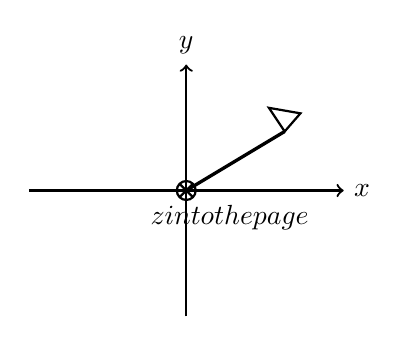
\begin{tikzpicture}[scale=1.0]
\draw[->,thick] (-2.0,0)--(2.0,0) node[right] {$x$};
\draw[->,thick] (0,-1.6)--(0,1.6) node[above] {$y$};
\draw[thick] (0,0) circle (0.12);
\draw[thick] (-0.08,-0.08)--(0.08,0.08);
\draw[thick] (-0.08,0.08)--(0.08,-0.08);
\draw[very thick] (0,0)--(1.25,0.75);
\draw[thick] (1.25,0.75)--(1.05,1.05)--(1.45,0.98)--cycle;
\draw (0.55,-0.35) node {$z\text{ into the page}$};
\end{tikzpicture}
\caption{A photon moving along the \(z\)-axis carries a transverse polarization ``flag'' in the \(xy\)-plane.}
\end{figure}

At first sight this sounds classical. One can imagine a little arrow or a little flag pointing somewhere in the plane. But the lecture is careful: the sentence ``the flag can point in any direction'' is only a provisional way of talking. It becomes correct only after we translate the story into quantum mechanics. The first task is not yet to quantize, but to understand how polarizers prepare and test such states.

Susskind reviews the standard wire-grid picture only as much as we need it. A grid can support currents in one direction and not in the orthogonal direction. As a result, one component of the electromagnetic field is reflected and the other passes through. Thus a polarizer prepares a transmitted wave whose electric field points along a definite axis. That transmitted axis, not the grid lines themselves, is the axis we use to label the polarization.

\section{Polarizers, Preparation, and the Conflict Between Symmetry and Discreteness}

Once we send photons one at a time through a polarizer, the apparatus plays two roles at once. It prepares a state and it measures a state. If a photon goes through a horizontal polarizer, we say it comes out horizontally polarized. If we then send it through a second horizontal polarizer, it goes through again. If instead we test it with a vertical polarizer, it does not go through.

So far there is nothing especially quantum mechanical here. A classical model with little flags or shaped bullets could mimic this kind of deterministic pass-or-block behavior. A fixed analyzer gives only two outcomes: pass or fail. Susskind lingers here on purpose. He wants us to feel that nothing mysterious has yet happened.

The mystery begins when symmetry is restored. If physics allows us to hold a polarizer horizontally or vertically, then by rotational symmetry it allows us to hold it at any intermediate angle. A photon can therefore be prepared at any angle in the \(xy\)-plane. But when we test that photon with a fixed polarizer, the outcome is still binary: pass or fail. The photon does not break into pieces, one piece transmitted and one piece absorbed. There are still only two outcomes.

\subsection{Question \& Answer}

\paragraph{Question.}
If polarization can point in any direction, why does a fixed measurement still return only two outcomes?

\paragraph{Answer.}
That is exactly the tension the lecture wants to isolate. On the one hand there is continuity: the preparation axis may be rotated through any angle. On the other hand there is discreteness: a fixed polarizer records only one of two outcomes. Quantum mechanics resolves this by abandoning the classical picture in which the intermediate polarization must already carry a definite pass-or-fail answer for every analyzer. Instead, a general state carries amplitudes, and the analyzer turns those amplitudes into probabilities. The continuum lies in the space of states; the discreteness lies in the outcomes of a chosen observable.

This is the point at which the lecture changes register. The physical story is not discarded, but it is no longer sufficient. We now need a two-dimensional state space.

\section{The \(x\)-\(y\) Basis and the First Observable}

We start with the simplest basis, horizontal and vertical polarization. Susskind calls them \(x\) and \(y\). Before writing vectors, he pauses over a small but important notation choice: polarization along a line has no preferred sign along that line. Horizontal-to-the-right and horizontal-to-the-left are the same polarization axis. That is why he draws a double arrow.

\begin{figure}
\centering

\includegraphics[width=0.32\textwidth]{lecture_06_figure_02.png}
\par
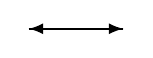
\begin{tikzpicture}[scale=1.0]
\draw[-latex,thick] (0,0)--(1.2,0);
\draw[-latex,thick] (1.2,0)--(0,0);
\end{tikzpicture}
\caption{The blackboard notation for a polarization axis: horizontal, but without a preferred left-versus-right direction.}
\end{figure}

With that convention in place we introduce the state vectors
\begin{equation}
|x\rangle=\begin{pmatrix}1\\0\end{pmatrix},
\qquad
|y\rangle=\begin{pmatrix}0\\1\end{pmatrix}.
\end{equation}
They are normalized,
\begin{equation}
\langle x|x\rangle=1,
\qquad
\langle y|y\rangle=1,
\end{equation}
and orthogonal,
\begin{equation}
\langle x|y\rangle=0.
\end{equation}

\begin{figure}
\centering

\includegraphics[width=0.55\textwidth]{lecture_06_figure_03.png}
\caption{Blackboard recap of orthogonality and the matrix action of the first polarization observable in the \(x,y\) basis.}
\end{figure}

The blackboard fragment above shows exactly the two facts Susskind wants to keep in view at once: orthogonality at upper left, and operator action in the main field. The visible matrix multiplication on the board is
\begin{equation}
\begin{pmatrix}
1&0\\
0&-1
\end{pmatrix}
\begin{pmatrix}
1\\
0
\end{pmatrix},
\end{equation}
and the natural completion of that displayed step is
\begin{equation}
\begin{pmatrix}
1&0\\
0&-1
\end{pmatrix}
\begin{pmatrix}
1\\
0
\end{pmatrix}
=
\begin{pmatrix}
1\\
0
\end{pmatrix}.
\end{equation}

Now we define the first observable. The physical measurement is simple: send the photon through an \(x\)-polarizer, write \(+1\) if it goes through, write \(-1\) if it does not. The numerical values \(+1\) and \(-1\) are conventional; they are chosen for symmetry and convenience. The operator is determined by its action on the basis states:
\begin{equation}
\hat P_{xy}|x\rangle=+|x\rangle,
\qquad
\hat P_{xy}|y\rangle=-|y\rangle.
\end{equation}
In the \((|x\rangle,|y\rangle)\) basis this means
\begin{equation}
P_{xy}=
\begin{pmatrix}
1&0\\
0&-1
\end{pmatrix}.
\end{equation}

This is the first place where the lecture makes the basic postulate concrete. An observable has eigenvectors and eigenvalues. The eigenvectors are the states in which the quantity is definite. The eigenvalues are the definite outcomes.

There is also already a small warning here. The column vectors themselves are not sacred objects in isolation. They are fixed only up to overall sign, and later up to overall phase. What is physically robust are the probabilities extracted from inner products.

\section{Rotated Linear Polarizations}

\subsection{The \(45^\circ\) basis}

The next move is as controlled as possible. Rotate the polarizer by \(45^\circ\). The outgoing photon is neither \(x\)-polarized nor \(y\)-polarized. Since the angle is exactly halfway between the two, Susskind motivates the state as having equal probabilities to pass an \(x\)-analyzer or a \(y\)-analyzer. That suggests
\begin{equation}
|/\rangle=\frac{1}{\sqrt2}\bigl(|x\rangle+|y\rangle\bigr)
=
\frac{1}{\sqrt2}
\begin{pmatrix}
1\\
1
\end{pmatrix}.
\end{equation}
The orthogonal companion may be taken as
\begin{equation}
|\backslash\rangle=\frac{1}{\sqrt2}\bigl(|x\rangle-|y\rangle\bigr)
=
\frac{1}{\sqrt2}
\begin{pmatrix}
1\\
-1
\end{pmatrix}.
\end{equation}
The sign choice is not important; the lecture explicitly notes that one could put the minus sign on either component. What matters is orthogonality:
\begin{equation}
\langle /|\backslash\rangle
=
\frac12-\frac12
=
0.
\end{equation}

Now the standard measurement rule appears in its simplest nontrivial form. The amplitude to find the photon in the \(x\)-eigenstate is
\begin{equation}
\langle x|/\rangle=\frac{1}{\sqrt2},
\end{equation}
so the probability that a \(45^\circ\)-prepared photon passes an \(x\)-polarizer is
\begin{equation}
|\langle x|/\rangle|^2=\frac12.
\end{equation}
Likewise
\begin{equation}
|\langle y|/\rangle|^2=\frac12.
\end{equation}

At the moment when the slash/backslash observable is written, the transcript is partially garbled. But the operator consistent with the stated eigenvectors and eigenvalues is naturally
\begin{equation}
P_{/\backslash}=
\begin{pmatrix}
0&1\\
1&0
\end{pmatrix},
\end{equation}
since
\begin{align}
P_{/\backslash}
\begin{pmatrix}
1\\
1
\end{pmatrix}
&=
\begin{pmatrix}
1\\
1
\end{pmatrix},
&
P_{/\backslash}
\begin{pmatrix}
1\\
-1
\end{pmatrix}
&=
-
\begin{pmatrix}
1\\
-1
\end{pmatrix}.
\end{align}
This is the first clear example of a state being definite for one observable and only probabilistic for another. The point is not that some quantities are observable and others are not. All of them are observable. The point is that a given state determines which observable is definite.

\subsection{Arbitrary angle \(\theta\)}

Once the \(45^\circ\) case is clear, the general angle is almost forced on us. If the polarization axis is rotated by an angle \(\theta\) from horizontal, then the corresponding unit vector has components \(\cos\theta\) and \(\sin\theta\). Thus
\begin{equation}
|\theta\rangle=\cos\theta\,|x\rangle+\sin\theta\,|y\rangle
=
\begin{pmatrix}
\cos\theta\\
\sin\theta
\end{pmatrix}.
\end{equation}
The orthogonal direction is \(\theta+\pi/2\), so
\begin{equation}
|\theta+\pi/2\rangle
=
-\sin\theta\,|x\rangle+\cos\theta\,|y\rangle
=
\begin{pmatrix}
-\sin\theta\\
\cos\theta
\end{pmatrix}.
\end{equation}
These vectors are normalized because \(\cos^2\theta+\sin^2\theta=1\), and they are orthogonal because
\begin{equation}
\langle \theta|\theta+\pi/2\rangle
=
\cos\theta(-\sin\theta)+\sin\theta\cos\theta
=
0.
\end{equation}

Now let us ask the operational question: if a photon is prepared by a \(\theta\)-polarizer, what is the probability that it passes an \(x\)-polarizer? The amplitude is
\begin{equation}
\langle x|\theta\rangle=\cos\theta,
\end{equation}
so
\begin{equation}
P(\theta\to x)=|\langle x|\theta\rangle|^2=\cos^2\theta.
\end{equation}
Likewise
\begin{equation}
P(\theta\to y)=|\langle y|\theta\rangle|^2=\sin^2\theta.
\end{equation}
The two probabilities add to \(1\), as they must.

\begin{figure}
\centering
\begin{tikzpicture}[scale=1.0]
\draw[->,thick] (-0.8,0)--(7.8,0);
\draw[thick,rotate around={25:(1,0)}] (1,-1)--(1,1);
\draw[thick,rotate around={70:(5,0)}] (5,-1)--(5,1);
\draw (1,-1.35) node {$\alpha$};
\draw (5,-1.35) node {$\beta$};
\draw (3.0,0.45) node {$|\alpha\rangle$};
\end{tikzpicture}
\caption{A photon prepared by an \(\alpha\)-polarizer is tested by a second polarizer at angle \(\beta\).}
\end{figure}

The lecture then inserts a short trigonometric interlude, not as a separate topic but because the physics now requires it. For the general two-polarizer experiment we need only
\begin{align}
\cos(\alpha-\beta)&=\cos\alpha\cos\beta+\sin\alpha\sin\beta,\\
\cos 2\theta&=\cos^2\theta-\sin^2\theta,\\
\sin 2\theta&=2\sin\theta\cos\theta.
\end{align}
If the first polarizer prepares
\begin{equation}
|\alpha\rangle=
\begin{pmatrix}
\cos\alpha\\
\sin\alpha
\end{pmatrix},
\qquad
\langle \beta|=
\begin{pmatrix}
\cos\beta&\sin\beta
\end{pmatrix},
\end{equation}
then the amplitude to pass the second polarizer is
\begin{equation}
\langle\beta|\alpha\rangle
=
\cos\alpha\cos\beta+\sin\alpha\sin\beta
=
\cos(\alpha-\beta).
\end{equation}
The transmission probability is therefore
\begin{equation}
P(\alpha\to\beta)=|\langle\beta|\alpha\rangle|^2=\cos^2(\alpha-\beta).
\end{equation}

This is the familiar law, but in the lecture it arrives with a very specific pedagogical payoff. The answer depends only on the relative angle, as symmetry demands, yet the outcome of any individual trial remains discrete. The inner product is the amplitude; the squared modulus is the probability.

\section{Intermediate Polarizers and the Observable \(P_\theta\)}

After the break the lecture resumes with a student question. This is an excellent place to preserve the tension-and-resolution structure explicitly.

\subsection{Question \& Answer}

\paragraph{Question.}
How can adding another polarizer increase the chance of transmission?

\paragraph{Answer.}
Suppose a photon gets through a \(\theta\)-polarizer. It is then in the state \(|\theta\rangle\). If we test it immediately with a \(\theta+\pi/2\) polarizer, the transmission probability is
\begin{equation}
P(\theta\to \theta+\pi/2)=\cos^2(\pi/2)=0.
\end{equation}
So the direct channel is closed.

Now insert a horizontal polarizer in between. First the photon must pass the horizontal polarizer:
\begin{equation}
P(\theta\to x)=\cos^2\theta.
\end{equation}
But if it does pass, the state is no longer \(|\theta\rangle\). This is the crucial update rule. Successful passage through the middle polarizer prepares a new state, namely \(|x\rangle\). The probability that this new state then passes the last polarizer is
\begin{equation}
P(x\to \theta+\pi/2)=\sin^2\theta.
\end{equation}
Therefore the total probability is the product of successive conditional probabilities:
\begin{equation}
P(\theta\to x\to \theta+\pi/2)=\cos^2\theta\,\sin^2\theta.
\end{equation}

\begin{figure}
\centering
\begin{tikzpicture}[scale=1.0]
\draw[->,thick] (-0.8,0)--(8.8,0);
\draw[thick,rotate around={30:(1,0)}] (1,-1)--(1,1);
\draw[thick] (4,-1)--(4,1);
\draw[thick,rotate around={120:(7,0)}] (7,-1)--(7,1);
\draw (1,-1.35) node {$\theta$};
\draw (4,-1.35) node {$x$};
\draw (7,-1.55) node {$\theta+\pi/2$};
\end{tikzpicture}
\caption{The inserted horizontal polarizer prepares a new state. That is why the forbidden direct channel can reopen with nonzero probability.}
\end{figure}

The point is not that probabilities somehow add mysteriously when we insert obstacles. The point is that measurements change the state. Each successful polarizer prepares the photon anew.

With that puzzle resolved, Susskind returns to the operator for a general angle. We want an observable whose eigenvectors are \(|\theta\rangle\) and \(|\theta+\pi/2\rangle\), with eigenvalues \(+1\) and \(-1\):
\begin{equation}
\hat P_\theta|\theta\rangle=+|\theta\rangle,
\qquad
\hat P_\theta|\theta+\pi/2\rangle=-|\theta+\pi/2\rangle.
\end{equation}
The transcript and chalk algebra are partially garbled at this point, but the cleaned result is standard and is precisely the matrix that makes these two equations true:
\begin{equation}
P_\theta=
\begin{pmatrix}
\cos 2\theta & \sin 2\theta\\
\sin 2\theta & -\cos 2\theta
\end{pmatrix}.
\end{equation}

A short check captures the logic of the blackboard derivation. Write \(c=\cos\theta\) and \(s=\sin\theta\), so that
\begin{equation}
|\theta\rangle=
\begin{pmatrix}
c\\
s
\end{pmatrix}.
\end{equation}
Then
\begin{align}
P_\theta|\theta\rangle
&=
\begin{pmatrix}
c^2-s^2 & 2sc\\
2sc & s^2-c^2
\end{pmatrix}
\begin{pmatrix}
c\\
s
\end{pmatrix} \\
&=
\begin{pmatrix}
(c^2-s^2)c+2sc\,s\\
2sc\,c+(s^2-c^2)s
\end{pmatrix} \\
&=
\begin{pmatrix}
c(c^2+s^2)\\
s(c^2+s^2)
\end{pmatrix}
=
\begin{pmatrix}
c\\
s
\end{pmatrix}
=
|\theta\rangle.
\end{align}
The companion state \(|\theta+\pi/2\rangle\) is similarly sent to minus itself.

There is a useful corollary:
\begin{equation}
P_{\theta+\pi/2}=-P_\theta.
\end{equation}
Rotating the analyzer by \(90^\circ\) does not create a completely new observable; it simply interchanges the positive and negative eigenvalues.

\section{Complex Coefficients and Circular Polarization}

At this stage the lecture deliberately widens the state space. If we have discussed only real coefficients, then we have still not used one of the main ingredients of quantum mechanics: complex numbers. So we introduce a new state,
\begin{equation}
|c_+\rangle=\frac{1}{\sqrt2}
\begin{pmatrix}
1\\
i
\end{pmatrix},
\end{equation}
and its orthogonal partner
\begin{equation}
|c_-\rangle=\frac{1}{\sqrt2}
\begin{pmatrix}
1\\
-i
\end{pmatrix}.
\end{equation}
Normalization uses the complex conjugate:
\begin{equation}
\langle c_+|c_+\rangle=\frac12\bigl(1\cdot 1+(-i)\cdot i\bigr)=1,
\end{equation}
and orthogonality does too:
\begin{equation}
\langle c_-|c_+\rangle=\frac12\bigl(1\cdot 1+i\cdot i\bigr)=0.
\end{equation}

From the wave point of view, these are not just \(45^\circ\) linear polarizations in disguise. If
\begin{equation}
E_y=\cos(z-ct),
\qquad
E_x=\cos(z-ct),
\end{equation}
then the two components are in phase and we simply have linear polarization at \(45^\circ\). Circular polarization arises when the two components are out of phase by \(90^\circ\):
\begin{equation}
E_y=\cos(z-ct),
\qquad
E_x=\sin(z-ct),
\end{equation}
or with the opposite sign in the second equation. At a fixed point in space the electric field rotates in time. That is the wave picture behind the complex state vectors. The lecture calls these left and right circular polarization, but Susskind explicitly says he may have the handedness labels swapped, so we keep only the pair itself fixed.

Now let us test a circularly polarized photon with a linear polarizer at angle \(\theta\). Using
\begin{equation}
|\theta\rangle=
\begin{pmatrix}
\cos\theta\\
\sin\theta
\end{pmatrix},
\end{equation}
the amplitude is
\begin{equation}
\langle \theta|c_+\rangle
=
\frac{1}{\sqrt2}\bigl(\cos\theta+i\sin\theta\bigr).
\end{equation}
The probability is the modulus squared:
\begin{align}
|\langle \theta|c_+\rangle|^2
&=
\frac12\bigl(\cos\theta+i\sin\theta\bigr)\bigl(\cos\theta-i\sin\theta\bigr) \\
&=
\frac12\bigl(\cos^2\theta+\sin^2\theta\bigr)
=
\frac12.
\end{align}
So a circularly polarized photon passes any linear polarizer with probability \(1/2\). That is the real content used in the lecture. The larger family, with arbitrary complex coefficients, leads to elliptically polarized states, but the lecture only gestures in that direction and postpones the corresponding observables.

\section{Incompatible Polarizations and Average Value}

By now we have many observables: \(P_{xy}\), the slash/backslash observable, the general \(P_\theta\), and the circular polarization observable that is left as homework. The key structural fact is that different polarization observables generally do not commute. The reason is visible even before one writes commutators: they do not share eigenvectors. Horizontal/vertical eigenvectors, \(45^\circ\) eigenvectors, and circular eigenvectors are different bases of the same two-dimensional state space.

The special exception is the orthogonal pair \(\theta\) and \(\theta+\pi/2\). Their observables are negatives of one another:
\begin{equation}
P_{\theta+\pi/2}=-P_\theta.
\end{equation}
Hence they commute, and measuring one automatically tells us the other. But for genuinely different directions the observables are incompatible. One cannot have a polarizer that prepares definite \(x\)-polarization and definite \(\theta\)-polarization at the same time.

The lecture then makes one last pivot. We have been calculating probabilities. What about average values? Susskind immediately complains about the terminology: ``expectation value'' is a misnomer. The last thing one should expect in a single trial is often the expectation value itself.

\begin{figure}
\centering

\includegraphics[width=0.58\textwidth]{lecture_06_figure_04.png}
\par
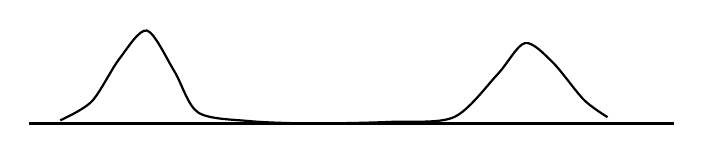
\begin{tikzpicture}[scale=1.0]
\draw[thick] (-4.1,0)--(4.1,0);
\draw[thick,smooth] plot coordinates {
(-3.7,0.04) (-3.3,0.28) (-2.95,0.82) (-2.6,1.18) (-2.25,0.66)
(-1.95,0.14) (-1.3,0.03) (-0.5,0.00) (0.5,0.02) (1.3,0.08)
(1.85,0.62) (2.2,1.02) (2.55,0.78) (2.95,0.30) (3.25,0.08)};
\end{tikzpicture}
\caption{The symmetric two-lump wavefunction used in the lecture to separate ``average'' from ``most likely measured value.''}
\end{figure}

The two-lump sketch above makes the point. A symmetric wavefunction with one lump at the left and one at the right can have
\begin{equation}
\langle x\rangle=0,
\end{equation}
even though the particle is least likely to be found near the middle. Thus the expectation value is an average value, not the value one should expect to see on an individual trial.

The general formula is derived by expanding a state in an eigenbasis of a Hermitian operator \(K\). If
\begin{equation}
K|n\rangle=\lambda_n|n\rangle,
\qquad
\sum_n |n\rangle\langle n|=I,
\end{equation}
then
\begin{align}
\langle K\rangle_\psi
&=
\langle \psi|K|\psi\rangle \\
&=
\left\langle \psi\left|K\left(\sum_n |n\rangle\langle n|\right)\right|\psi\right\rangle \\
&=
\sum_n \langle \psi|K|n\rangle\langle n|\psi\rangle \\
&=
\sum_n \lambda_n\,\langle \psi|n\rangle\langle n|\psi\rangle \\
&=
\sum_n \lambda_n\,|\langle n|\psi\rangle|^2.
\end{align}
This is exactly the weighted average of the possible measurement outcomes: eigenvalue times probability, summed over all outcomes.

For polarization the simplest example uses the original operator \(P_{xy}\) in the state \(|\theta\rangle\):
\begin{align}
\langle P_{xy}\rangle_\theta
&=
\langle \theta|P_{xy}|\theta\rangle \\
&=
\begin{pmatrix}
\cos\theta & \sin\theta
\end{pmatrix}
\begin{pmatrix}
1&0\\
0&-1
\end{pmatrix}
\begin{pmatrix}
\cos\theta\\
\sin\theta
\end{pmatrix} \\
&=
\cos^2\theta-\sin^2\theta \\
&=
\cos 2\theta.
\end{align}
This number lies between \(+1\) and \(-1\), as it must. But again, it is an average. It is not itself a third outcome of the measurement. The actual outcomes remain \(+1\) or \(-1\).

\section{Summary}

Photon polarization is the cleanest two-state quantum system precisely because it begins with such an innocent picture. A photon moving along \(z\) seems to carry only a little transverse flag. A polarizer seems to do nothing more mysterious than pass one orientation and block another. But symmetry immediately forces a continuum of preparation directions, while every fixed analyzer still returns only two outcomes. From there the lecture builds the whole elementary quantum structure: state vectors, orthogonal bases, observables, amplitudes, probabilities, state update under measurement, complex superpositions, incompatible observables, and finally average value. The system is small, but the logic is already the full logic of quantum mechanics.